\chapter{The Learn tab and the console}
\label{ch:learn}

\section{The Learn tab}
\key{F1} (or the orange \ui{Learn} button) opens the Learn tab; the Learning layout puts it beside the Scene view. Each
of its 45 lessons connects three layers: the Unity concept you can see on screen, the equivalent Blender concept with
the folder in Blender's source where it lives, and the theory behind it, cited from the reference books
\cite{MarschnerShirley2021, Gregory2018vol1, Gregory2018vol2} and the papers behind the features (the
\emph{References} lesson). Pick a lesson on the left; your progress is saved; \ui{Try it} buttons drive the editor for
you so you can watch the concept happen; click a question to reveal its answer; hover over almost any button or field
in the editor to see its Blender equivalent; the \ui{?} beside the status bar's hint opens the lesson for what you are
doing. Index C of this guide lists every lesson with its sources.

\begin{figure}[H]
  \centering
  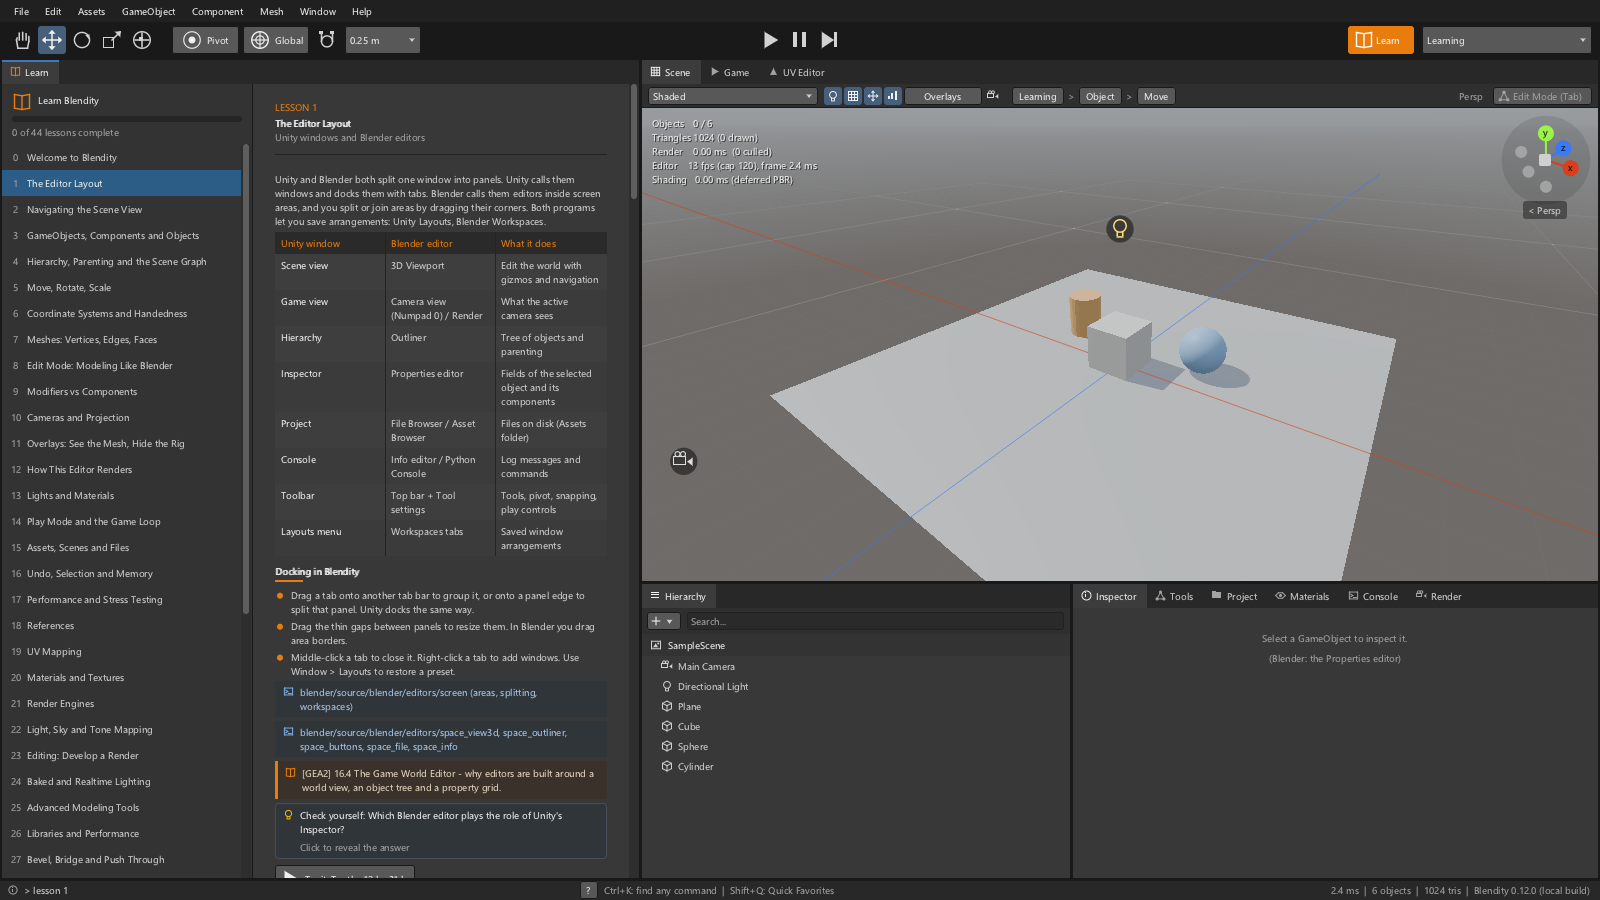
\includegraphics[width=\textwidth, alt={The Learning layout: the Learn tab's lesson list and a lesson with its table, references and Try-it buttons on the left, the Scene view the buttons drive on the right.}]{layout-learning.png}
  \caption{The Learning layout: the lesson list, a lesson with its table, references and Try-it buttons, and the Scene
  view the buttons drive.}
\end{figure}

The lessons, in order: Welcome to Blendity; The Editor Layout; Navigating the Scene View; GameObjects, Components and
Objects; Hierarchy, Parenting and the Scene Graph; Move, Rotate, Scale; Coordinate Systems and Handedness; Meshes:
Vertices, Edges, Faces; Edit Mode: Modeling Like Blender; Modifiers vs Components; Cameras and Projection; Overlays;
How This Editor Renders; Lights and Materials; Play Mode and the Game Loop; Assets, Scenes and Files; Undo, Selection
and Memory; Performance and Stress Testing; References; UV Mapping; Materials and Textures; Render Engines; Light, Sky
and Tone Mapping; Editing: Develop a Render; Baked and Realtime Lighting; Advanced Modeling Tools; Libraries and
Performance; Bevel, Bridge and Push Through; Rendering on the GPU; Points, Lines, N-gons and Booleans; Drawing in
Perspective; Customizing the Editor; Sculpting; Painting the Surface; The Hand-painted Look; Stylized Environments;
Drawing like SketchBook; Papers; Blender's Shader Nodes in the Textures Window; Fog with a Volume Material; Working
Faster with Textures and Materials; Flatten to the Camera; Shapes by the Camera's Angle; Animating Any Property; The Books and the References.

\section{The console}
Every tool can be driven from the Console's command line (type \code{help}; \key{Up} and \key{Down} recall what you
typed; a mistyped command is answered with the nearest known ones), which is also how scripts and the tests drive the
editor. None of it is needed any more: every verb an artist uses has a menu item, a button or a field. A few that are
handy by hand:

\begin{center}
\small
\begin{tabularx}{\textwidth}{lX}
\toprule
Command & Does \\
\midrule
\code{set Camera.FStop 1.4} & sets any field of the selected objects' components (enums by text) \\
\code{layout UV Unwrapping}, \code{alltools on} & layouts and Show All Tools \\
\code{skin bind}, \code{skin transfer Body Shirt} & automatic weights, weight transfer \\
\code{autorig humanoid}, \code{autorig build} & the marker auto-rig \\
\code{anim new}, \code{anim frame 30}, \code{anim record on}, \code{anim retarget <rig>} & the Animation window \\
\code{meshmaps 1024 16}, \code{surface new}, \code{paint on}, \code{smat apply Worn Steel} & the paint pipeline \\
\code{export textures unity Exports/Crate --assign} & the texture set packed for Unity, assigned to the material \\
\code{sketch on}, \code{sketchguide perspective 3}, \code{sketchcanvas ground}, \code{sketchbuild box} & the sketch pen, its guides and canvases, solids from the lines \\
\code{sculpt on}, \code{sculpt brush clay}, \code{sculpt dynamesh 128}, \code{sculpt remesh 2000} & Sculpt Mode and the remeshers \\
\code{render wait}, \code{saverender out.png}, \code{renderanim 1 120 24} & a render held till done, saved; an animation \\
\code{import <file>}, \code{export glb Exports/Hero.glb}, \code{export unitypackage <folder>} & files in and out \\
\code{livelink start}, \code{livelink status} & Live Link \\
\code{libs}, \code{jobs}, \code{budget pc}, \code{keymap table} & the build's libraries, the running jobs, the VRChat budget, every preset's keys \\
\code{update check}, \code{update history}, \code{update install <tag>} & the updater \\
\code{vr start}, \code{vr sketch on}, \code{vr paint on} & the VR View \\
\bottomrule
\end{tabularx}
\end{center}

\section{Headless runs and scripts}
\code{Blendity --headless-screenshot out.png --size 1600x900 --cmd "<command>" \ldots --frames N} runs the commands
with no window and writes a picture; \code{BLENDITY\_PROJECT} and \code{BLENDITY\_TRASH} point it at a scratch project,
never your \code{Assets}. The figures in this guide, the tests and the Unity comparison harness are made that way.

\section{Checking how it works for you}
\code{docs/hci/checklist.md} lists 118 tasks across the editor, each with its steps, what should happen and a target
time; its interactive page times each task with a stopwatch and keeps your results so the slow ones can be improved
first. How the editor's ease of use was measured (the keystroke-level model \cite{Card1980Keystroke}, the Fitts audit
\cite{Fitts1954Information}, the walkthroughs \cite{Polson1992Cognitive}, the heuristics \cite{Nielsen1994Enhancing}) is
in \code{docs/hci/README.md}.
